\documentclass{article}

\usepackage{dirtree}

\usepackage[
  height=9in,      % height of the text block
  width=7.5in,       % width of the text block
  top=78pt,        % distance of the text block from the top of the page
  headheight=48pt, % height for the header block
  headsep=12pt,    % distance from the header block to the text block
  heightrounded,   % ensure an integer number of lines
        % show the main blocks
  verbose,         % show the values of the parameters in the log file
]{geometry}
\setlength{\parindent}{0pt}
\usepackage{amsmath}
\usepackage{courier}
\usepackage{graphicx}
\usepackage{amsmath}
\usepackage{booktabs}
\usepackage{fancyhdr}
\usepackage{float}
\usepackage{mathtools}

\pagestyle{fancy}
\fancyhead[L]{Pattern and Speech Recognition WS1617\\ Assignment 10}
\fancyhead[R]{ Vinh Thinh Ho (2562630) \\ Noshaba Cheema (2562653)}

\renewcommand{\headrulewidth}{0.35pt}
\newcommand\tab[1][1cm]{\hspace*{#1}}

\begin{document}
\section*{Exercise 10.1}
a)\\
Largest eigenvalue of M (greatest absolute value) = -12 with corresponding eigenvector ($\frac{-1}{3}$, $\frac{-2}{3}$, $\frac{2}{3}$)

b) see \textbf{10.1.py}\\
c) The plot:
\begin{figure}[ht]
\centering
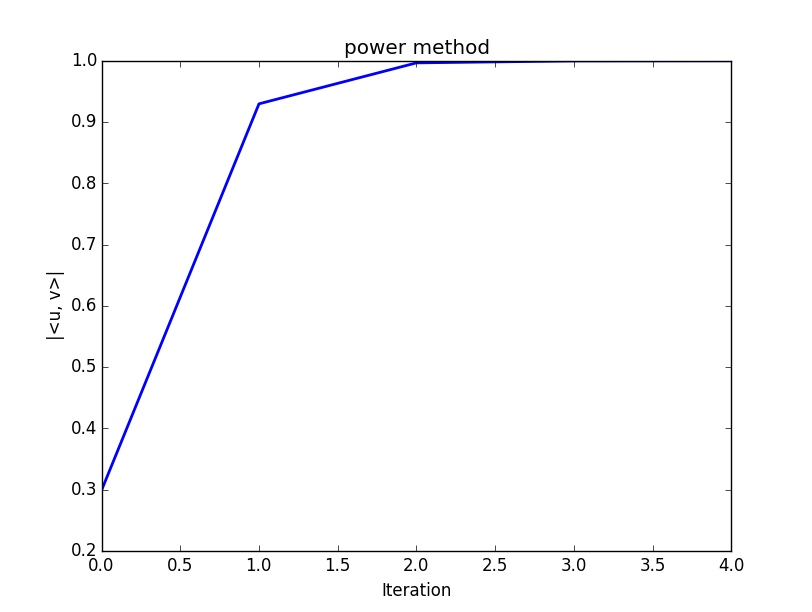
\includegraphics[scale=0.5]{101.png}
\end{figure}

\section*{Exercise 10.2}
a,b,c,d,e,f) see \textbf{10.2\_bonus.py}\\
The plot:
\begin{figure}[ht]
\centering
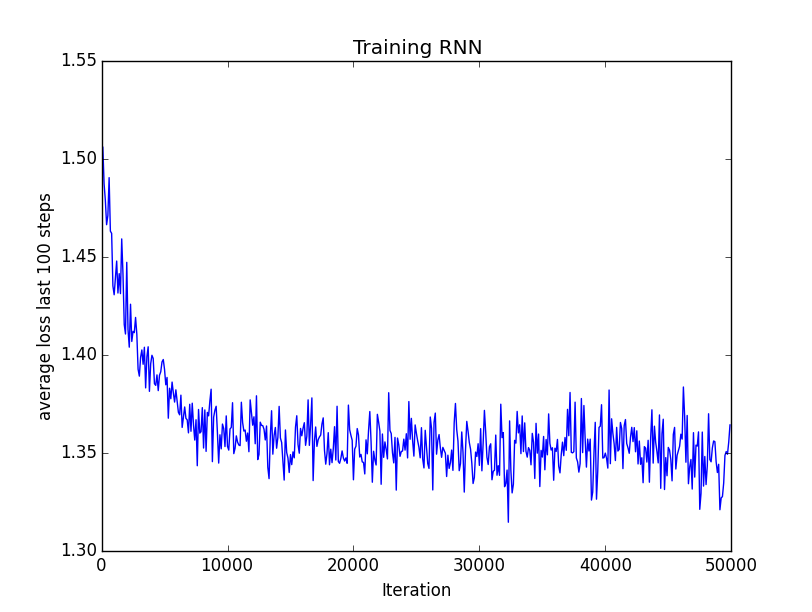
\includegraphics[scale=0.5]{102.png}
\end{figure}

\section*{Bonus}
a) see \textbf{10.2\_bonus.py} \\

Achieved perplexity when testing on the whole sequence: $\approx$ 3.83 
\\\\
b) We can see that the perplexity is almost 4, so this model will predict the sequence almost randomly, which is not good. But, this is reasonable because the input data is also almost randomly.
\\\\
Let's look at the second data set that we created "data2.txt":\\\\
"aaaaaaaaaa...cccccccccc...gggggggggg...tttttttttt..."\\\\
in which each nucleotide is repeated 100 times. We have following result:\\

\begin{figure}[ht]
\centering
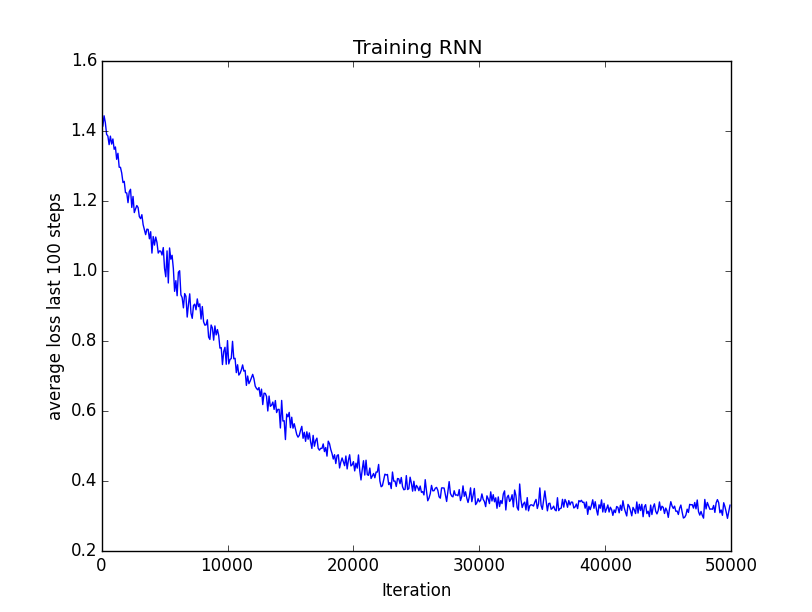
\includegraphics[scale=0.5]{bonus.png}
\end{figure}

Perplexity for this data set: $\approx$ 1.06, which is very good, because the input has a clear pattern.


\end{document}



